\chapter{Hands-On Tools from Locally Available Materials} 

Mathematics is a hands-on subject. Students must touch one-half, straight lines, negative numbers, circles, squares, cylinders, decimals, numbered items and shapes, and all other concepts in order to learn mathematics properly. There is a limitless number of items that can be made to teach mathematics. These items can be made from local materials, frequently from left-over materials so that there is no additional cost in money.

Each tool is explained in terms of how to make and then how to use. If science needs local materials and student-centered learning to discover, then math, as the core of science, must be taught in the same manner. Every science syllabus uses mathematics!

\section{Accounts} \label{accountstools}
\textbf{How to Make:} Use large manila posters to make T-accounts tables. Make removable paper strips with tape to place transactions under the debit (Dr) or credit (Cr) sides, and account headings (Capital, Sales, Purchases, etc.) for opening new accounts.\\

\noindent\textbf{Uses:}
\begin{itemize}
\item Students physically place and move items to show cash flow among the different accounts.
\item Use a paper or toy bus, the Transaction Express, to demonstrate the double entry rule of book-keeping.
\item See more in Topics and Activities for the Form III topic of \nameref{accountsactivities}.
\end{itemize}

\section{Cartesian Plane} \label{cartesianplane}
\textbf{How to Make:} Use an empty seed bag (mfuko), a sheet of manila paper or a wire grid to draw a large Cartesian plane with $x$ and $y$ axes. Points can be little dots or bottle caps with tape on the back, which can easily be moved around. Then connect with string for lines, etc.\\

\noindent\textbf{Uses:}
\begin{itemize}
\item Create \nameref{dice} that can be used to plot random points. Make four dice out of manila paper (2 red - one of +'s and -'s and one of the numbers 1 - 6, and then 2 blue in the same way). Students roll the dice to find an $x$-coordinate (blue) and a $y$-coordinate (red) and then must plot the point on the Cartesian plane. Use this method to generate coordinate points for problems on slope, equation of a line, midpoint, distance formula, etc.
\item Students are challenged by plotting $(1,0)$; $(0,1)$ and many such points, so practice and drilling are essential before trying to teach functions or relations.
\item One can find the midpoint or any other properties of a line segment. Leaving a Cartesian plane in the classroom, students can use it during private studies. The tangible Cartesian plane is so essential because a 2-dimensional plane needs tangible interaction for learning.
\item A reusable Cartesian plane saves much time in the classroom compared to drawing it on the board each time you teach a concept. Accuracy is so essential in teaching midpoint and related topics.
\end{itemize}

\section{Circles} \label{circlestools}
\textbf{How to Make:} Use bike wheels or bucket lids to draw circles on the board. Have students use coins or toilet paper rolls to draw them in their notebooks.\\

\noindent\textbf{Uses:}
\begin{itemize}
\item Wrap string around the wheel or lid to show circumference. Use another string to measure diameter, and use the ratio of the lengths to derive $\pi$. Compare results from different groups in class.
\item Students can use a wheel to find the perimeter around the school or their home.
\item See more in Topics and Activities for the Form III topic of \nameref{circlesactivities}.
\end{itemize}

\section{Clinometer} \label{clinometer}
\textbf{How to Make:} Gather a protractor, a hollow pen tube or straw, a short piece of string (15 cm), some tape and a nail or some other small weight.

Tie the weight to one end of the string and tie the other end around the center of the pen tube. Tape the pen tube along the straight edge of the protractor so that the string hangs vertically downward through the center (make sure it is secured in place).\\

\noindent\textbf{Uses:}
\begin{itemize}
\item \emph{Trigonometry}: The clinometer can be used to find the height of a tree or tall building. A student stands some distance away from the tree or building and looks through the pen tube so that he\slash she can see the highest point of the object. Another student reads the angle made by the string with the vertical $90^\circ$ line on the protractor. (Note that when reading an angle $\theta$ from the protractor, the value $(90^\circ - \theta)$ should be used since the string bob starts vertically downward at $90^\circ$ rather than $0^\circ$.) Knowing the horizontal distance from the student to the object, as well as the height of the student by using a tape measure, one can use the properties of trigonometry to calculate the height of the object!

Help students to prepare a data table as shown below, and then split them up into groups to go collect and record their data and calculate the height of a building. Have them compare their answers and identify sources of error. If possible, obtain the actual height and see how the calculated values compare. This is a great Math Practical for Form IV students! What kind of professions might use this method of measurement?
\end{itemize}

\section{Compass} \label{compass}
\textbf{How to Make:} Use a strip of folded paper with holes at various lengths along the paper. Keep one pen secure at one end and use another pen or pencil to trace a circle. Alternatively, use two pens with a length of string tied around each one. Unroll the connecting string to the desired length and secure one pen to be the center of the circle and use the other to trace the circumference.\\

\noindent\textbf{Uses:}
\begin{itemize}
\item Have each student make one of these paper compasses for taking notes, especially during topics when they need to draw many, many circles. Otherwise they will be sharing coins or compasses and it will take a long time for them to copy your notes.
\end{itemize}

\section{Dice} \label{dice}
\textbf{How to Make:} Take an empty chalk container and write numbers on the sides. Or you can make a box using manila paper, or even make cubes out of bars of soap. Have your students help to make them - they love helping with these projects.\\

\noindent\textbf{Uses:}
\begin{itemize}
\item \emph{Probability}: Students love to play and see probability happen rather than just memorizing formulas. Chart the results of using dice. Then discover the formulas of probability.
\item \emph{Coordinate Geometry}: Use dice to generate random numbers for plotting points, graphing lines, etc.
\item \emph{Numbers}: Use random numbers to drill students on multiplication, addition, fractions, decimals, etc.
\end{itemize}

\section{Dominoes} \label{dominoes}
\textbf{How to Make:} Use a little rectangular paper marked in 2 sections. For example, one section has a number four and the other section has a number six.\\

\noindent\textbf{Uses:}
\begin{itemize}
\item From the example, the ordered pair $(4,6)$ can be written. This random point can be graphed on a \nameref{cartesianplane}.
\item These domino cards can also be used for random pairing of numbers as they learn multiplication tables. These must be drilled in many ways, because older students often still use tables on their exercise books, which will not be available to them during exams.
\end{itemize}

\section{Flash Cards} \label{flashcards}
\textbf{How to Make:} Small cards or paper rectangles can be used.\\

\noindent\textbf{Uses:}
\begin{itemize}
\item Students enjoy playing \nameref{aroundtheworld} in the classroom as multiplication tables are drilled.
\item These cards can be used for board races with 6 or more students at the board responding to the flash card. All the students at their desks can also be responding to the question.
\item Use flashcards with pictures or math terms written on them to quiz students on new terminology.
\end{itemize}

\section{Fractions and Decimals} \label{fracsanddecs}
\textbf{How to Make:} Empty water bottles are excellent for teaching fractions and are very meaningful. Each student can supply an empty bottle from home to use during class.

Sticks can be put to better use in math class than for discipline. Have the students collect them and they will become fractions. Now the students have an object of one-half, one-third or any fractional component. After students understand these fraction concepts, there are activities on \nameref{fractions} which may be used. \\

\noindent\textbf{Uses:}
\begin{itemize}
\item Have students fill up half a bottle, one-third of a bottle, etc. Students can continue to add one-half and one-half to get a full bottle as they work together in pairs with their bottles of water.
\item Students can then subtract with fractions in the same way. What learning! Have them write all the fraction addition and subtraction problems they have solved. Creating fraction equations with the sticks and then solving them will help the students understand the operations on fractions.
\item Relating these fractions to cooking will be very practical and meaningful. To cook, one measures one cup, a half cup, a third cup, etc. What happens when we must cook for twice the number of people?
\item Convert these learning exercises to decimals. Students need to see and touch 0.5 or 0.3 or 0.25 to learn the meaning of it. Sometimes even money can be used.
\end{itemize}

\section{Geoboard} \label{geoboard}
\textbf{How to Make:} Gather nails and left-over square slabs of wood of various sizes from a local carpenter, or have students supply these items from their homes. Place nails in a grid at one inch or 2 centimeters apart from each other, across and down to get a square. The number of nails used will be based on the size of the piece of wood. A size of 10 by 10 is excellent. 

Many times a carpenter will share these items to increase the learning experience of students, or your school may share. The carpenter knows how often numbers are used in his profession! Every student can build a geoboard, or one geoboard for a group of 4 students. It is good to involve the parents in a day school.\\

\noindent\textbf{Uses:}
\begin{itemize}
\item \emph{Perimeter}: The formula for perimeter around any size rectangle can be demonstrated. For example, for a rectangle of 5 inches by 4 inches, one can use rubber bands to mark off the given dimensions, and then one can count 18 units of perimeter to see that:\\
\begin{center}
$2 \times \text{Length} + 2 \times \text{Width} = \text{Perimeter}$
\end{center}
\item \emph{Area}: The formula for area can be demonstrated by marking a rectangle of 5 inches by 4 inches or any dimension. Use rubber bands to mark the square. Count the square units in the surface of the rectangle - it will be 20 square units. This will allow students to discover the formula:\\
\begin{center}
$\text{Length} \times \text{Width} = \text{Area} $
\end{center}
\item \emph{Coordinate Geometry}: Lines can be graphed on a \nameref{cartesianplane}. First mark the $x$-axis and $y$-axis. It is good to use different colors of rubber bands (yellow for $y$-axis and red for $x$-axis). Use little dots of paper to plot the points. After plotting 3 or 4 points, use a rubber band to connect them. The students enjoy such hands on activities.

After a line is plotted, one can demonstrate slope, or gradient. Slope is the change of $y$ over change of $x$ and can be counted and demonstrated on a geoboard.

Parallel lines can be placed on a geoboard with rubber bands. Then one can use the points to see that the slopes are equal for these two lines. Also try it with perpendicular lines.
\item \emph{Relations and Functions}: After tables of values are created, students can plot them on the geoboard. Begin by graphing the line using two points from the table. Then one can find the domain and range. The inverse can be discovered and discussed as well. All of this on relations can also be applied to functions.
\end{itemize}

\section{Globe} \label{globe}
\textbf{How to Make:} Have students make spheres by binding thin strips of bamboo together with string. Make sure they have axes through the center and a few outer rings. You can fill in the empty sections with paper to illustrate various angles within the sphere.\\

\noindent\textbf{Uses:}
\begin{itemize}
\item \emph{Earth as a Sphere}: Use the spheres in class to teach students about longitude and latitude, great circles, the equator and prime meridian, and various angles measured within the sphere. Color-code different properties and have students try to label them.
\end{itemize}

\section{Number Line} \label{numberline}
\textbf{How to Make:} Create a number line in a variety of ways. The best may be a piece of string or ruler. Then have numbers written on little dots that can be placed along the number line in positive and negative directions.

Students can be a number line in class. Thy can hold a positive or negative number. Involvement is the best way to learn. 

Number lines can be drawn outside in the dirt for even more interactive learning.\\

\noindent\textbf{Uses:}
\begin{itemize}
\item Use the ``hopping method'' of movement as students process $-3 + 1 = -2$. Have one student at a time stand in front of the student number line and hop to the left and right to add and subtract integers. It is good to create a hopping song while learning these negative integers for addition and subtraction. 
\item Inequalities are graphed on a \nameref{numberline}. These graph are the stepping stone to graphing on an $x$-$y$ plane. It also demonstrates which numbers are larger or smaller. Students need to see to understand such concepts of greater than or less than.
\end{itemize}

\section{Protractor} \label{protractor}
\textbf{How to Make:} Take a square piece of paper and fold it in half into two vertical rectangles (picture 1). Take the top right corner and fold it down to the center line (picture 2). Next, bring the bottom left corner to the same point on the center line so that the left edge meets along the edge just folded (not pictured). Then fold up the lower edge to make the bottom triangle (picture 3). Finally tuck the bottom triangle inside (picture 4). Leave the triangle folded like this, or unfold (picture 5) to view the angles created. Label the angles as shown - this protractor produces angles of $15^\circ$, $30^\circ$, $45^\circ$, $60^\circ$, $75^\circ$, $90^\circ$, $120^\circ$ and $135^\circ$.

	\begin{center}
	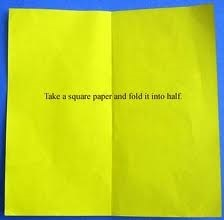
\includegraphics[width=5cm]{./img/prot1.jpg}
	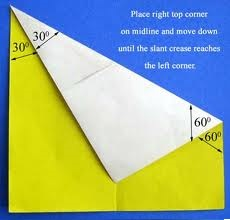
\includegraphics[width=5cm]{./img/prot2.jpg}
	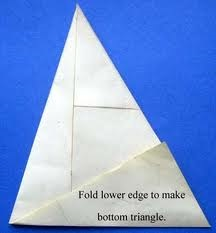
\includegraphics[width=5cm]{./img/prot3.jpg}
	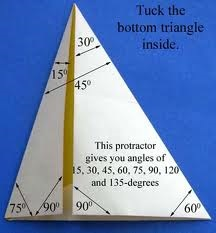
\includegraphics[width=5cm]{./img/prot4.jpg}
	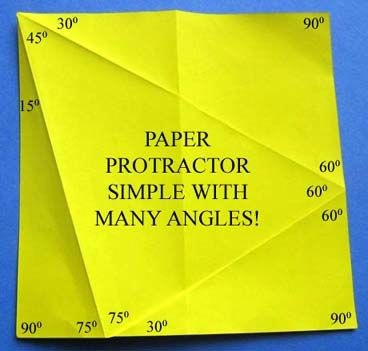
\includegraphics[width=5cm]{./img/prot5.jpg}
	\end{center}

\noindent\textbf{Uses:}
\begin{itemize}
\item \emph{Geometry}: Students can use the paper protractor to construct various acute, obtuse, right and reflex angles.
\end{itemize}

\section{Three-Dimensional Objects} \label{3dfigstools}
\textbf{How to Make:} Use paper or a wire grid to construct cylinders, prisms and pyramids. Use empty cardboard boxes or chalk boxes to demonstrate interior angles formed by various planes. Use old Nido tins as cylinders.\\

\noindent\textbf{Uses:}
\begin{itemize}
\item Students get great enjoyment out of constructing these three-dimensional objects themselves. Use them to derive formulas on surface area and volume.
\item Tape a sheet of paper around a large cylindrical tin and use circular lids to show how to derive the surface area of a cylinder.
\item See more in Topics and Activities for the Form IV topic of \nameref{3dfigsactivities}.
\end{itemize}